%-------------------------------------------------------------------------------
% Edge detectors review
% by Haldo Spontón & Juan Cardelino
% IPOL 2012
%-------------------------------------------------------------------------------
\documentclass{ipol}
\ipolSetYear{2012}
\ipolSetDOI{10.XXXX/ipol.2012.sc-red}

\usepackage{hyperref,verbatim,graphicx,amsmath,amssymb,amssymb,dsfont}
\usepackage[ruled,linesnumbered]{algorithm2e}
\usepackage{sidecap,subfig,array}
\usepackage[table]{xcolor}
\usepackage{multicol}
\newtheorem{theorem}{Theorem}
\numberwithin{equation}{section}
\numberwithin{table}{section}
\numberwithin{figure}{section}
\begin{document}

%-------------------------------------------------------------------------------
\title{Review of Edge Detectors}
\author{Haldo Spont\'on,\\
        Juan Cardelino}
\date{}
\ipolMaketitle

%-------------------------------------------------------------------------------
\begin{ipolAbstract}
In this paper we study some of the classic alternatives for edge detection in digital images. The main idea 
behind the edge detection is to find where there are abrupt changes in the intensity of an image. 
As a first approach, the first derivative is used to find the changes of intensity in several algorithms 
such as Sobel, Prewitt and Roberts. The second derivative is also used, for example in algorithms 
like Marr-Hildreth and Haralick.\\
We compare the results obtained from a qualitative point of view (perceptual) and from a quantitative 
point of view (number of operations, execution time), considering different forms to convolve an 
image with a kernel (step required in some of the algorithms).\\


%The Marr-Hildreth algorithm is a method of detecting edges in digital 
%images. It's based on convolving the image with the Laplacian of the 
%Gaussian function. Then, zero crossings are detected in the filtered 
%result to obtain the edges points.
\end{ipolAbstract}

%-------------------------------------------------------------------------------
\begin{ipolCode}
The C implementation of the algorithms implemented in this work (beta version) can be
downloaded from:
\begin{itemize}
	\item Roberts, Prewitt and Sobel operators: \href{http://iie.fing.edu.uy/~haldos/ipol/fded.tar.gz}{here}.
	\item Marr-Hildreth algorithm: \href{http://iie.fing.edu.uy/~haldos/ipol/marr-hildreth.tar.gz}{here}.
	\item Haralick algorithm: \href{http://iie.fing.edu.uy/~haldos/ipol/haralick.tar.gz}{here}.
\end{itemize}
\end{ipolCode}

%-------------------------------------------------------------------------------
%\begin{ipolSupp}
%\end{ipolSupp}

%-------------------------------------------------------------------------------
\section{Introduction}
\label{sec:intro}

Edge detection is one of the first approaches published in the literature for 
segmenting images. The basic idea is to detect abrupt changes in intensity. 
Detecting those changes in intensity for the purpose of finding edges in images 
can be accomplished using first or second order derivatives. 

In the 70's, edge detection methods were based on using small operators 
(such as Sobel masks), attempting to compute an approximation of the
first derivative of the image. In section ~\ref{sec:first} we study the 
performance of such algorithms, as an introduction to a more sophisticated 
analysis into the edge finding process.\\

In 1980 Marr and Hildreth argued that intensity changes are not independent 
of image scale, so the edge detection requires the use of different size 
operators. They also argued that a sudden intensity change will be seen 
as a peak (or trough) in the first derivative or, equivalently, as a zero 
crossing in the second derivative. The bulk of this work focuses on the 
study of this algorithm, presented in Section ~\ref{sec:second}.\\

In section ~\ref{sec:examples} we present some examples to compare the 
performance of the algorithms studied in this work. We also present a 
video created using the Marr-Hildreth algorithm, applied frame by frame.\\

%-------------------------------------------------------------------------------
\section{Algorithms based on first derivative}
\label{sec:first}

The selected tool to find the amplitude and direction of changes in 
intensity of an image $f$ is the gradient operator (denoted as $\nabla$), defined 
as the vector:
\begin{equation}
	\nabla f = 
				\begin{bmatrix} 
					g_x \\ g_y
				\end{bmatrix}
	=				
				\begin{bmatrix} 
					\cfrac{\partial f}{\partial x} \\ \cfrac{\partial f}{\partial y} \\
				\end{bmatrix}
\end{equation}

The magnitude ($M$) and direction ($\alpha$) of the gradient vector $\nabla f$ at location $(x,y)$
are calculated as:
\begin{equation}
	\begin{cases}
		M(x,y) = \sqrt{g_x^2 + g_y^2} \\
		\alpha(x,y) = \tan^{-1} \begin{bmatrix} g_x \\ g_y \end{bmatrix} \\
	\end{cases}
\end{equation}

The direction of an edge at an arbitrary location $(x,y)$ of the image is 
orthogonal to the direction $\alpha(x,y)$ of the gradient vector.\\

We need to compute partial derivatives $\partial f/\partial x$ and $\partial f/\partial y$ 
at every pixel in the image. Since we are dealing with digital images, numerical approximations 
of the partial derivatives over a neighborhood about a point are required. Next we will study 
the methods of Roberts, Prewitt and Sobel, whose main difference is how they approach this calculation.\\

\subsection{The \textit{Roberts} operators}

The most usual approach of the first derivative is to take the Taylor expansion of order zero with
a small $h$. Approximating the first derivative:
\begin{equation}
	f'(x) \simeq \frac{f(x+h) - f(x)}{h}\\
\end{equation}
The image has discrete points of coordinates $(i,j)$, so taking $x=i*h$ and $y=j*h$, we approximate the 
first derivative of the image based on the intensity values ​​at points of the image as:
\begin{equation}
\label{eq:roberts1}
	g_x = \frac{\partial f(x,y)}{\partial x} = f(x+1,y) - f(x,y)
\end{equation}
and
\begin{equation}
\label{eq:roberts2}
	g_y = \frac{\partial f(x,y)}{\partial y} = f(x,y+1) - f(x,y)\\
\end{equation}

Equations \ref{eq:roberts1} and \ref{eq:roberts2} can be implemented for all values of $x$ and $y$
by filtering the image $f(x,y)$ with the 1-D masks in figure \ref{fig:1dmasks}. But when we want 
to find diagonal edges, we need 2-D masks. The \textit{Roberts operators} are one of the earliest 
attempts to use 2-D masks with this purpose. These operators are based on implementing the diagonal 
diferences implemented by filtering an image with the masks in figure \ref{fig:roberts}.\\

\begin{SCfigure}[3][!h]
	\centering
	\includegraphics[width=0.14\textwidth]{1dmasks.pdf}
	\caption{One-dimensional masks used to implement equations \ref{eq:roberts1} and \ref{eq:roberts2}.}
	\label{fig:1dmasks}
\end{SCfigure}

\begin{SCfigure}[3][!h]
	\centering
	\includegraphics[width=0.15\textwidth]{roberts.pdf}
	\caption{\textit{Roberts cross-gradient} 2-D masks.}
	\label{fig:roberts}
\end{SCfigure}

\subsection{The \textit{Prewitt} operators}

Masks of size $2\times2$ are conceptually simple, but not being symmetrical to a central point implies 
that they are not as useful for detecting edges as symmetrical ones. The smaller mask with these characteristics is 
$3\times3$. These masks provide more information to find the direction of the edges, because they take 
into account information on opposite sides of the central point.\\

The simplest digital approximation to the partial derivatives using masks of size $3\times3$ are given 
by taking the difference between the third and first rows (or columns) of the $3\times3$ region. The
difference between the third and first rows approximates the derivative in the x-direction, and 
the difference between the third and first columns approximates the derivative in the y-direction.
These approximations can be implemented by filtering the image with the two masks in figure \ref{fig:prewitt}.
These masks are called \textit{Prewitt operators}.\\

\begin{SCfigure}[2][!h]
	\centering
	\includegraphics[width=0.25\textwidth]{prewitt.pdf}
	\caption{\textit{Prewitt} 2-D masks of size $3\times3$.}
	\label{fig:prewitt}
\end{SCfigure}

\subsection{The \textit{Sobel} operators}

A slight variation of the Prewitt operators use more weight on the central coefficients of the 
difference. It can be shown that using a $2$ in the center location provides image smoothing. This
variation is implemented using masks in figure \ref{fig:sobel}. These operators are called 
\textit{Sobel operators}.\\

\begin{SCfigure}[2][!h]
	\centering
	\includegraphics[width=0.25\textwidth]{sobel.pdf}
	\caption{\textit{Sobel} 2-D masks of size $3\times3$.}
	\label{fig:sobel}
\end{SCfigure}

The Prewitt masks are simpler to implement than the Sobel masks, but the computational difference
between them is not an issue. It is preferable to use Sobel operators, because they have better
noise-suppression characteristics (smoothing). Noise suppression is an important issue when dealing
with derivatives.\\

%-------------------------------------------------------------------------------
\section{Algorithms based on second derivative}
\label{sec:second}

The edge detection methods discussed in the previous section are simply based on filtering the 
image with different masks, without taking into account the characteristics of the edges or 
noise in the image.\\

The two algorithms that we will see in this section (Marr-Hildreth [1980] and Haralick [1987]) 
are based on the second derivative of the image, and both take steps to reduce noise before 
detecting edges in the image.\\

\subsection{The \textit{Marr} and \textit{Hildreth} algorithm}

The Marr-Hildreth algorithm is a method of detecting edges in digital 
images. It's based on find zero crossing points of the second derivative
of the image. This can be done in several ways. In this work we implemented 
two different ways; convolving the image with a Gaussian kernel and then 
approximating the second derivative (Laplacian) with a 3x3 kernel, or 
convolving the image with a kernel calculated as the Laplacian of a 
Gaussian function. There are more ways to do so, for example, using 
recursive Gaussian filters.\\ % poner referencia!

The algorithm is divided in three steps, each one described later:
\begin{enumerate}
	\item Grayscale conversion of the input image (see section \ref{sec:appendix1}).
	\item Convolution of the image with:
	\begin{itemize}
		\item a Laplacian of Gaussian (LoG) kernel. (or)
		\item a Gaussian kernel and then a Laplacian operator.
	\end{itemize}
	\item Search of zero crossing points in the filtered image.\\
\end{enumerate}

Some auxiliary functions were implemented for computing the operations
needed in the algorithm, such as Gaussian kernel and Laplacian of a Gaussian 
kernel generation, and 2-D convolution of an image with a given kernel, 
with zero padding.\\



%-------------------------------------------------------------------------------
\subsubsection{Gaussian and LoG kernels}

The Marr-Hildreth algorithm consists of convolving the LoG filter with an input image, $f(x,y)$.
\begin{equation}\label{eq:log}
  g(x,y) = [\nabla^2G(x,y)]\star f(x,y)
\end{equation}
and then finding the zero crossings of $g(x,y)$ to determine the location of edges in $f(x,y)$. 
Because these are linear processes, equation \ref{eq:log} can be written also as
\begin{equation}
  g(x,y) = \nabla^2[G(x,y)\star f(x,y)]
\end{equation}
indicating that we can smooth the image first with a Gaussian filter and then compute the Laplacian of the result.\\

Then we need to generate both Gaussian kernel and LoG kernel (see section \ref{sec:appendix2}).\\

The Marr-Hildreth edge-detection algorithm may be summarized as follows:
\begin{enumerate}
	\item Filter the input image with a $n \times n$ Gaussian lowpass filter obtained by sampling equation \ref{eq:gaussian_function}.
	\item Compute the Laplacian of the image resulting from step 1, using, for example, the $3\times3$ mask:
			$\begin{bmatrix}
			1 &  1 & 1 \\
			1 & -8 & 1 \\
			1 &  1 & 1 \\
			\end{bmatrix}$\footnote{Steps 1 and 2 can be made into one, using a $n\times n$ LoG lowpass filter obtained by sampling equation \ref{eq:log_function}.}
	\item Find the zero crossings of the image from step 2.
\end{enumerate}

%-------------------------------------------------------------------------------
\subsubsection{Zero crossing}

A zero crossing at pixel $p$ implies that the signs of at least two opposite neighboring pixels are 
different. There are four cases to test: left/right, up/down, and the two diagonals. In this case 
we work with a threshold, so that not only the signs of the opposite pixels must differ, also their 
difference in absolute value must be greater than a certain threshold.\\

Zero crossing detection is the key feature of the Marr-Hildreth edge detection method. The technique 
presented in the previous paragraph is attractive for its simplicity of implementation and its low 
computational cost. In general it is a technique that yields good results, but if more precision in 
finding the zero crossings is needed, methods for finding zero crossings with subpixel accuracy 
should be used.\\

%-------------------------------------------------------------------------------
\subsection{The \textit{Haralick} algorithm}

The idea behind the Haralick edge detector is identical to that of the previous method; find zeros in 
the second derivative of the image. In this method, we smooth the input image through local bi-cubic
polynomial fitting. Then, calculating the second derivative analytically, we can find an expression 
equivalent to cancel the second derivative of the polynomial as a function of the parameters of it.\footnote{This implementation is slightly 
different to the traditional implementation of the Haralick algorithm. We do not use the condition concerning the third derivative.}\\

\subsubsection{Bi-cubic polynomial fitting}
\label{sec:bicubic}

We adjust the surrounding neighborhood of a point $(x,y)$ in the image $f$ using the following bi-cubic polynomial:
\begin{equation}
	\label{eq:bicubic}
	f(x,y) = k_1 + k_2x + k_3y + k_4x^2 + k_5xy + k_6y^2 + k_7x^3 + k_8x^2y + k_9xy^2 + k_{10}y^3\\
\end{equation}

To solve this problem, we need to take more neighbors than coefficients to be adjusted. The smallest 
neighborhood of odd dimensions has size $5\times5$. Now it is possible to convolve the input image
with some precomputed masks, instead of finding the least square solution to find the coefficients 
$k_1\dots k_{10}$ at each point $(x,y)$.\\

Consider 25 points in a small neighborhood of a point $(x,y)$ in the image. We use a least square
formulation to obtain the coefficients (25 points give equal number of equations):

\begin{equation*}
	\begin{array}{l}
		f_1 = f(x_1,y_1) = k_1 + k_2x_1 + k_3y_1 + k_4x_1^2 + k_5x_1y_1 + k_6y_1^2 + k_7x_1^3 + k_8x_1^2y_1 + k_9x_1y_1^2 + k_{10}y_1^3\\
		f_2 = f(x_2,y_2) = k_1 + k_2x_2 + k_3y_2 + k_4x_2^2 + k_5x_2y_2 + k_6y_2^2 + k_7x_2^3 + k_8x_2^2y_2 + k_9x_2y_2^2 + k_{10}y_2^3\\
		\vdots \\
		f_{25} = f(x_{25},y_{25}) = k_1 + k_2x_{25} + k_3y_{25} + k_4x_{25}^2 + k_5x_{25}y_{25} + k_6y_{25}^2 + k_7x_{25}^3 + k_8x_{25}^2y_{25} + k_9x_{25}y_{25}^2 + k_{10}y_{25}^3\\
	\end{array}
\end{equation*}

Using matrix notation:

\begin{equation*}
	\begin{bmatrix} 
		f_1		\\ 
		f_2		\\ 
		\vdots	\\
		f_{25}
	\end{bmatrix} 
	= 
	\begin{bmatrix} 
		1 		& x_1 		& y_1 		& x_1^2 	& x_1y_1 		& y_1^2 	& \hdots 	& y_1^3 	\\
		1 		& x_2 		& y_2 		& x_2^2 	& x_2y_2 		& y_2^2 	& \hdots 	& y_2^3 	\\
		\vdots	& \vdots	& \vdots	& \vdots	& \vdots		& \vdots	& \ddots	& \vdots	\\
		1 		& x_{25}	& y_{25}	& x_{25}^2 	& x_{25}y_{25} 	& y_{25}^2 	& \hdots 	& y_{25}^3
	\end{bmatrix}
	\times
	\begin{bmatrix}
		k_1		\\
		k_2		\\
		\vdots	\\
		k_{10}
	\end{bmatrix}
	\Rightarrow \mathbf{f} = \mathbf{A}\mathbf{k}\\
\end{equation*}

Then:

\begin{equation*}
	(\mathbf{A}^T\mathbf{A})^{-1}\mathbf{A}^T\mathbf{f} = \mathbf{k} \ \ \Rightarrow \ \ \mathbf{k} = \mathbf{B}\mathbf{f}\\
\end{equation*}

$\mathbf{B}$ is a $10\times25$ matrix: 

\begin{equation*}
	\begin{bmatrix}
		b_{1,1}		& b_{1,2}	& \hdots	& b_{1,25}	\\
		b_{2,1}		& b_{2,2}	& \hdots	& b_{2,25}	\\
		\vdots		& \vdots	& \ddots	& \vdots	\\
		b_{10,1}	& b_{10,2}	& \hdots	& b_{10,25}
	\end{bmatrix}
	\times
	\begin{bmatrix}
		f_1		\\
		f_2		\\
		\vdots	\\
		f_{25}
	\end{bmatrix}
	=
	\begin{bmatrix}
		k_1		\\
		k_2		\\
		\vdots	\\
		k_{10}
	\end{bmatrix}\\
\end{equation*}

For each coefficient ($i$ from $1$ to $10$):

\begin{equation}
	\label{eq:coefficients}
	k_i = b_{i,1}f_1 + b_{i,2}f_2 + b_{i,3}f_3 + \hdots + b_{i,25}f_{25} \ \ \Rightarrow \ \ \mathbf{k_i} = \mathbf{f}\star\mathbf{b_i}\\
\end{equation}

where:

\begin{equation}
	\label{eq:b_i}
	\mathbf{b_i} = \begin{bmatrix}	b_{i,1}		& b_{i,2}	& \hdots	& b_{i,5}	\\
									b_{i,6}		& b_{i,7}	& \hdots	& b_{i,10}	\\
									\vdots		& \vdots	& \ddots	& \vdots	\\
									b_{i,21}	& b_{i,22}	& \hdots	& b_{i,25}	\\
					\end{bmatrix}\\
\end{equation}

Using equation \ref{eq:coefficients} and the masks given in table \ref{table:b_i}, we can compute 
the coefficients $k_1 \hdots k_{10}$ for all the points in the image. The elements of the mask $\mathbf{b_i}$ 
are the elements of the i-th row of $\mathbf{B} = (\mathbf{A}^T\mathbf{A})^{-1}\mathbf{A}^T$.\\

\newcolumntype{C}{>{\centering\arraybackslash}m{1cm}<{}}
\begin{table}
\centering
\subfloat[$\mathbf{b_1}$.] {
\begin{tabular}{|*{5}{C|}}
\hline
425 & 275 & 225 & 275 & 425 \\
\hline
275 & 125 &  75 & 125 & 275 \\ 
\hline
225 &  75 &  25 &  75 & 225 \\
\hline
275 & 125 &  75 & 125 & 275 \\
\hline
425 & 275 & 225 & 275 & 425 \\
\hline
\end{tabular}}
\qquad\qquad
\subfloat[$\mathbf{b_2}$.] {
\begin{tabular}{|*{5}{C|}}
\hline
-2260 & -620 & 0 & 620 & 2260 \\ 
\hline
-1660 & -320 & 0 & 320 & 1660 \\ 
\hline
-1460 & -220 & 0 & 220 & 1460 \\
\hline
-1660 & -320 & 0 & 320 & 1660 \\ 
\hline
-2260 & -620 & 0 & 620 & 2260 \\
\hline
\end{tabular}} \\
\subfloat[$\mathbf{b_3}$.] {
\begin{tabular}{|*{5}{C|}}
\hline
2260  &  1660 &  1460 &  1660 &  2260 \\ 
\hline
620   &   320 &   220 &   320 &   620 \\ 
\hline
0     &     0 &     0 &     0 &     0 \\
\hline
-620  &  -320 &  -220 &  -320 &  -620 \\ 
\hline
-2260 & -1660 & -1460 & -1660 & -2260 \\
\hline
\end{tabular}}
\qquad\qquad
\subfloat[$\mathbf{b_4}$.] {
\begin{tabular}{|*{5}{C|}}
\hline
1130 & 620 & 450 & 620 & 1130 \\ 
\hline
830  & 320 & 150 & 320 &  830 \\ 
\hline
730  & 220 &  50 & 220 &  730 \\
\hline
830  & 320 & 150 & 320 &  830 \\ 
\hline
1130 & 620 & 450 & 620 & 1130 \\
\hline
\end{tabular}} \\
\subfloat[$\mathbf{b_5}$.] {
\begin{tabular}{|*{5}{C|}}
\hline
-400 & -200 & 0 &  200 &  400 \\ 
\hline
-200 & -100 & 0 &  100 &  200 \\ 
\hline
0    &    0 & 0 &    0 &    0 \\
\hline
200  &  100 & 0 & -100 & -200 \\ 
\hline
400  &  200 & 0 & -200 & -400 \\
\hline
\end{tabular}}
\qquad\qquad
\subfloat[$\mathbf{b_6}$.] {
\begin{tabular}{|*{5}{C|}}
\hline
1130 & 830 & 730 & 830 & 1130 \\ 
\hline
620  & 320 & 220 & 320 &  620 \\ 
\hline
450  & 150 &  50 & 150 &  450 \\
\hline
620  & 320 & 220 & 320 &  620 \\ 
\hline
1130 & 830 & 730 & 830 & 1130 \\
\hline
\end{tabular}} \\
\subfloat[$\mathbf{b_7}$.] {
\begin{tabular}{|*{5}{C|}}
\hline
-8260 & -2180 & 0 & 2180 & 8260 \\ 
\hline
-6220 & -1160 & 0 & 1160 & 6220 \\ 
\hline
-5540 &  -820 & 0 &  820 & 5540 \\
\hline
-6220 & -1160 & 0 & 1160 & 6220 \\ 
\hline
-8260 & -2180 & 0 & 2180 & 8260 \\
\hline
\end{tabular}}
\qquad\qquad
\subfloat[$\mathbf{b_8}$.] {
\begin{tabular}{|*{5}{C|}}
\hline
5640  &  3600 &  2920 &  3600 &  5640 \\ 
\hline
1800  &   780 &   440 &   780 &  1800 \\ 
\hline
0     &     0 &     0 &     0 &     0 \\
\hline
-1800 &  -780 &  -440 &  -780 & -1800 \\ 
\hline
-5640 & -3600 & -2920 & -3600 & -5640 \\
\hline
\end{tabular}} \\
\subfloat[$\mathbf{b_9}$.] {
\begin{tabular}{|*{5}{C|}}
\hline
-5640 & -1800 & 0 & 1800 & 5640 \\ 
\hline
-3600 &  -780 & 0 &  780 & 3600 \\ 
\hline
-2920 &  -440 & 0 &  440 & 2920 \\
\hline
-3600 &  -780 & 0 &  780 & 3600 \\ 
\hline
-5640 & -1800 & 0 & 1800 & 5640 \\
\hline
\end{tabular}}
\qquad\qquad
\subfloat[$\mathbf{b_{10}}$.] {
\begin{tabular}{|*{5}{C|}}
\hline
8260  &  6220 &  5540 &  6220 &  8260 \\ 
\hline
2180  &  1160 &   820 &  1160 &  2180 \\ 
\hline
0     &     0 &     0 &     0 &     0 \\
\hline
-2180 & -1160 &  -820 & -1160 & -2180 \\ 
\hline
-8260 & -6220 & -5540 & -6220 & -8260 \\
\hline
\end{tabular}} \\
\caption{Masks to compute the coefficients of the bicubic fit.}
\label{table:b_i}
\end{table}
\clearpage

\subsubsection{Analytical calculation of the second derivative}
\label{sec:secderivative}

We approximate the neighborhood of each point of the image using the bi-cubic polynomial 
expression in equation \ref{eq:bicubic}. If we just take the first order terms of this 
polynomial, the Gradient angle, defined with positive y-axis is defined as:

\begin{align}
\label{eq:sincos}
	\sin(\theta) & = \frac{k_2}{\sqrt{k_2^2 + k_3^2}} \nonumber \\
	\cos(\theta) & = \frac{k_3}{\sqrt{k_2^2 + k_3^2}} \nonumber \\
\end{align}

Now substituting the variables $x$ and $y$ in polar form as:

\begin{equation*}
	x = \rho\cos{\theta} \: , \: y = \rho\sin(\theta) \\
\end{equation*}

in the bi-cubic polynomial, we obtain:

\begin{equation}
	f_{\theta}(\rho) = C_0 + C_1\rho + C_2\rho^2 + C_3\rho^3
\end{equation}

where:

\begin{align}
\label{eq:c}
	C_0 & = k_1 \nonumber \nonumber \\
	C_1 & = k_2\sin(\theta) + k_3\cos(\theta) \nonumber \\
	C_2 & = k_4\sin^2(\theta) + k_5\sin(\theta)\cos(\theta) + k_6\cos^2(\theta) \nonumber \\
	C_3 & = k_7\sin^3(\theta) + k_8\sin^2(\theta)\cos(\theta) + k_9\sin(\theta)\cos^2(\theta) + k_{10}\cos^3(\theta). \nonumber \\
\end{align}

The derivatives are obtained as follows:

\begin{align}
	f'{\theta}(\rho) = C_1 + 2C_2\rho + 3C_3\rho^2 \nonumber \\
	f''{\theta}(\rho) = 2C_2 + 6C_3\rho \nonumber \\
\end{align}

Then, the condition of the second derivative equal to zero becomes:

\begin{equation}
	f''{\theta}(\rho) = 2C_2 + 6C_3\rho = 0 \ \ \Rightarrow \ \ \left| \frac{C_2}{3C_3} \right| < \rho_0.
\end{equation}

\subsubsection{Algorithm}

The Haralick edge detection algorithm is summarized in the following 4 steps:

\begin{enumerate}
	\item Find the coefficients $k_1 \hdots k_{10}$, as shown in section \ref{sec:bicubic}.
	\item Compute $\sin(\theta)$ and $\cos(\theta)$ (equations \ref{eq:sincos}).
	\item Compute $C_2$ and $C_3$ (equations \ref{eq:c}).
	\item If $\left| \frac{C_2}{3C_3} \right| < \rho_0$, then that point is an edge point.
\end{enumerate}

%-------------------------------------------------------------------------------
\section{Results}
\label{sec:results}

First we see the results of each of the algorithms on a simple test image, the white square on black background shown in figure \ref{fig:original1}. \\

\begin{figure}[h!]
	\centering
	\includegraphics[width=0.2\textwidth]{results/square.png}
	\caption{Test image 1: white square on black background.}
	\label{fig:original1}
\end{figure}

The figures \ref{fig:result1-a} to \ref{fig:result1-f} show the output of each algorithm. The first three correspond to the first derivative methods (Roberts, Prewitt and Sobel), then the following two are from the Marr-Hildreth algorithm using Gaussian and LoG kernels, and the last one corresponds to the Haralick algorithm. Execution time\footnote{Running on Intel Core i3 CPU (2.53GHz), 3 Gb RAM, standard laptop.} for each algorithm are shown in Table \ref{exectime1}. \\

\begin{figure}[h!]
	\centering
	\subfloat[Roberts.]{\label{fig:result1-a}\hspace*{0.5cm}\includegraphics[width=0.2\textwidth]{results/square_roberts.png}\hspace*{0.5cm}}
	\quad
	\subfloat[Prewitt.]{\label{fig:result1-b}\hspace*{0.5cm}\includegraphics[width=0.2\textwidth]{results/square_prewitt.png}\hspace*{0.5cm}}
	\quad
	\subfloat[Sobel.]{\label{fig:result1-c}\hspace*{0.5cm}\includegraphics[width=0.2\textwidth]{results/square_sobel.png}\hspace*{0.5cm}}

	\subfloat[Marr-Hildreth (Gaussian).]{\label{fig:result1-d}\hspace*{0.5cm}\includegraphics[width=0.2\textwidth]{results/square_marr-hildreth.png}\hspace*{0.5cm}}
	\quad
	\subfloat[Marr-Hildreth (LoG).]{\label{fig:result1-e}\hspace*{0.5cm}\includegraphics[width=0.2\textwidth]{results/square_marr-hildreth-log.png}\hspace*{0.5cm}}
	\quad
	\subfloat[Haralick.]{\label{fig:result1-f}\hspace*{0.5cm}\includegraphics[width=0.2\textwidth]{results/square_haralick.png}\hspace*{0.5cm}}
	\caption{Results of the algorithms using the figure \ref{fig:original1} as input image.}
	\label{fig:result1}
\end{figure}

\begin{table}[t!]
	\begin{center}
	\begin{tabular}{| l | r |}
		\hline \rule{0pt}{3ex}
		\cellcolor[gray]{0.8} \textbf{Algorithm}	& \cellcolor[gray]{0.8} \textbf{Execution time (s)}	\\ \hline \rule{0pt}{3ex}
		Roberts, Prewitt and Sobel					& $0.020 \ s$										\\ \hline \rule{0pt}{3ex}
		Marr-Hildreth (Gaussian)					& $0.030 \ s$										\\ \hline \rule{0pt}{3ex}
		Marr-Hildreth (LoG)							& $0.050 \ s$										\\ \hline \rule{0pt}{3ex}
		Haralick									& $0.040 \ s$										\\
		\hline
	\end{tabular}
	\end{center}
	\caption{Execution time of the algorithms using the figure \ref{fig:original1} as input image (128$\times$128 pixels, 1 channel).}
	\label{exectime1}
\end{table}
\vspace{0.5cm}

It is appreciated that in the simplest cases, the first derivative edge detection algorithms are running better and faster. Let us now analyze the performance of each of the algorithmos using a more realistic test image, shown in figure \ref{fig:original2}. \\

\begin{figure}[t!]
	\centering
	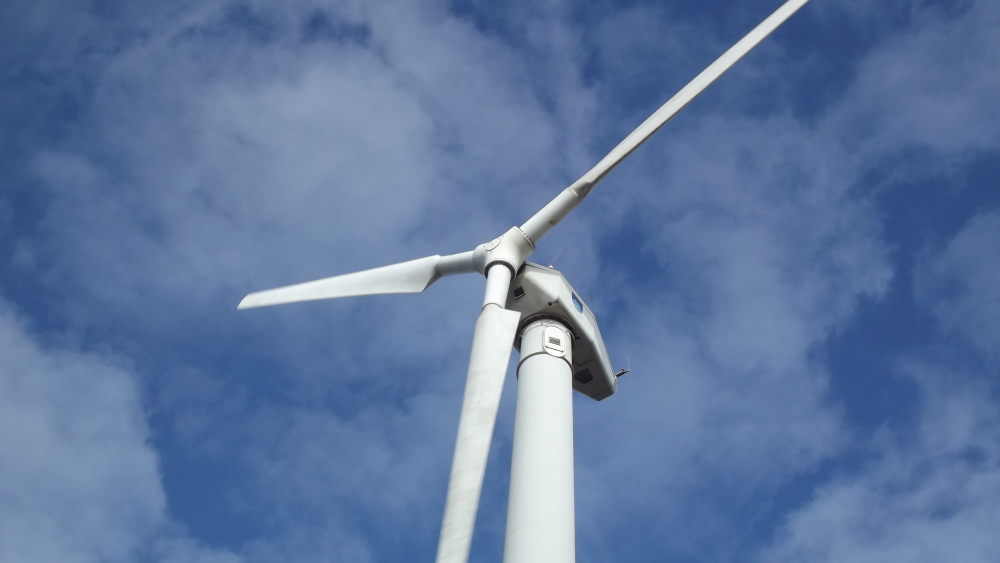
\includegraphics[width=0.5\textwidth]{results/molino.jpg}
	\caption{Test image 2: windmill.}
	\label{fig:original2}
\end{figure}

First we show in figure \ref{fig:result2} the results of the first derivative edge detection algorithms.

\begin{figure}[h!]
	\centering
	\subfloat[Roberts.]{\label{fig:result2-a}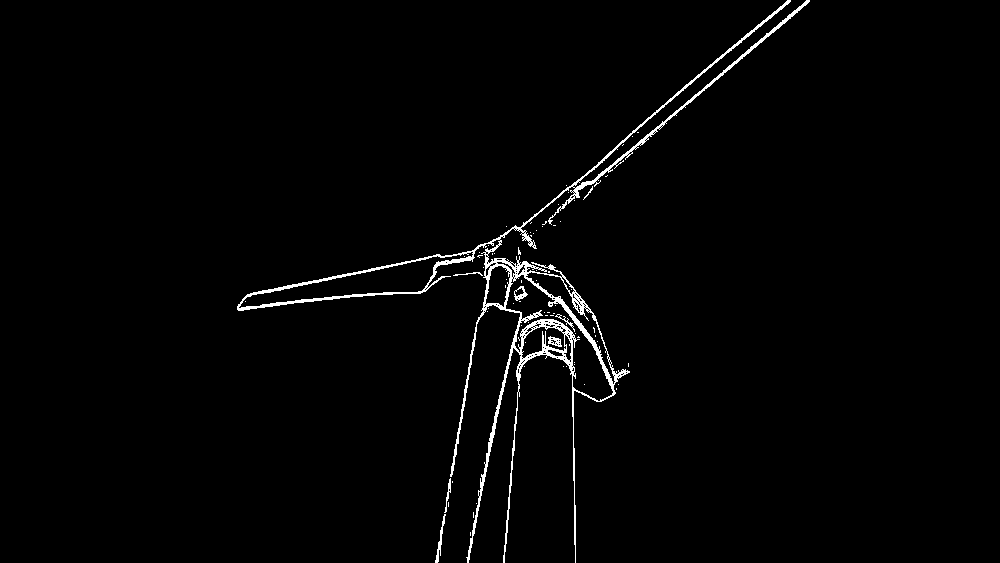
\includegraphics[width=0.42\textwidth]{results/molino_roberts.png}}
	\quad
	\subfloat[Prewitt.]{\label{fig:result2-b}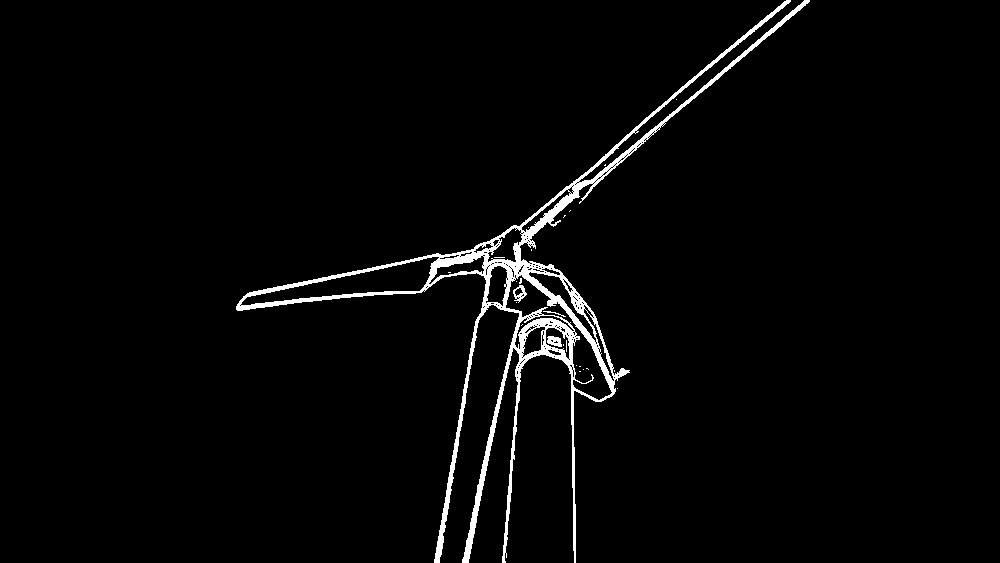
\includegraphics[width=0.42\textwidth]{results/molino_prewitt.png}}
	
	\subfloat[Sobel.]{\label{fig:result2-c}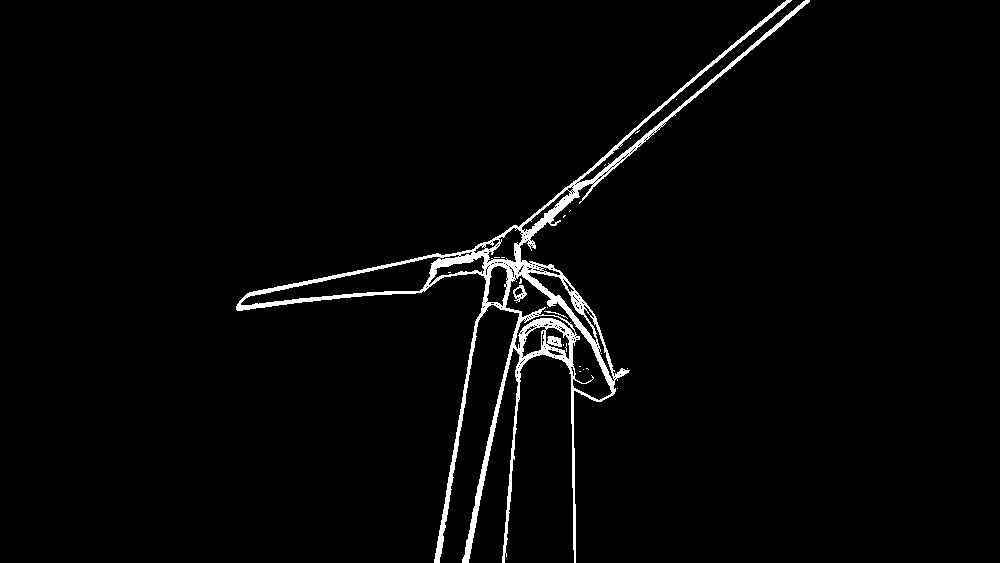
\includegraphics[width=0.42\textwidth]{results/molino_sobel.png}}
	\caption{Results of the first derivative algorithms using the figure \ref{fig:original2} as input image.}
	\label{fig:result2}
\end{figure}

Now we show in figures \ref{fig:result3-a} and \ref{fig:result3-b} the results obtained using the Marr-Hildreth algorithm (both Gaussian and LoG kernels), and in figure \ref{fig:result3-c} the results obtained using the Haralick algorithm. In table \ref{exectime2} we show the execution time for each one of the algorithms. \\

\begin{figure}[h!]
	\centering
	\subfloat[Marr-Hildreth (Gaussian).]{\label{fig:result3-a}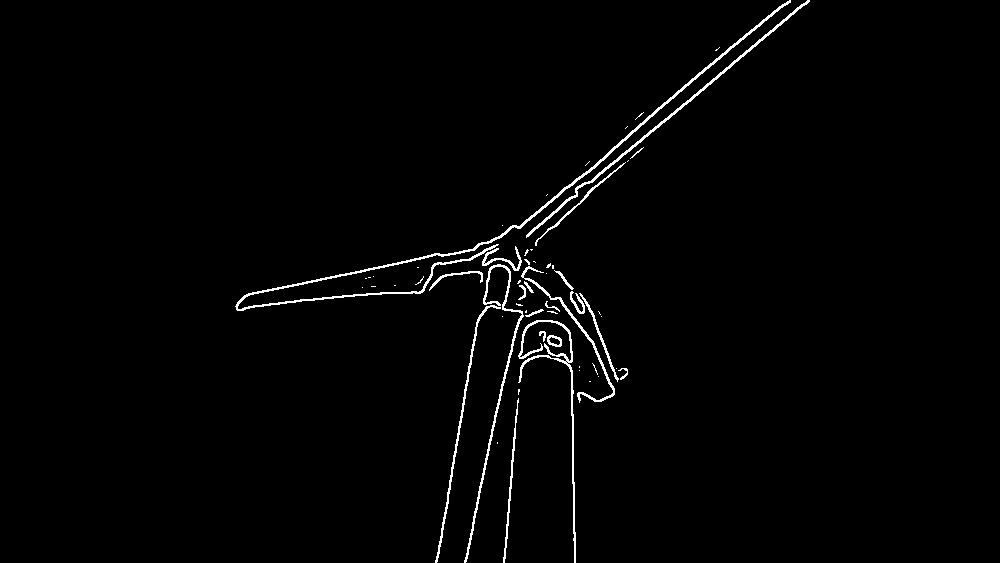
\includegraphics[width=0.42\textwidth]{results/molino_marr-hildreth.png}}
	\quad
	\subfloat[Marr-Hildreth (LoG).]{\label{fig:result3-b}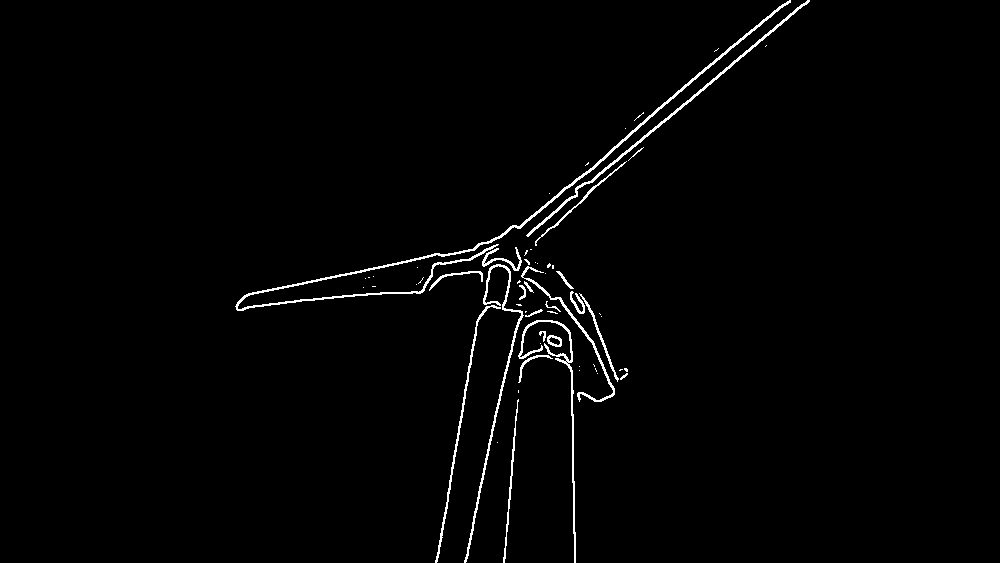
\includegraphics[width=0.42\textwidth]{results/molino_marr-hildreth-log.png}}
	
	\subfloat[Haralick.]{\label{fig:result3-c}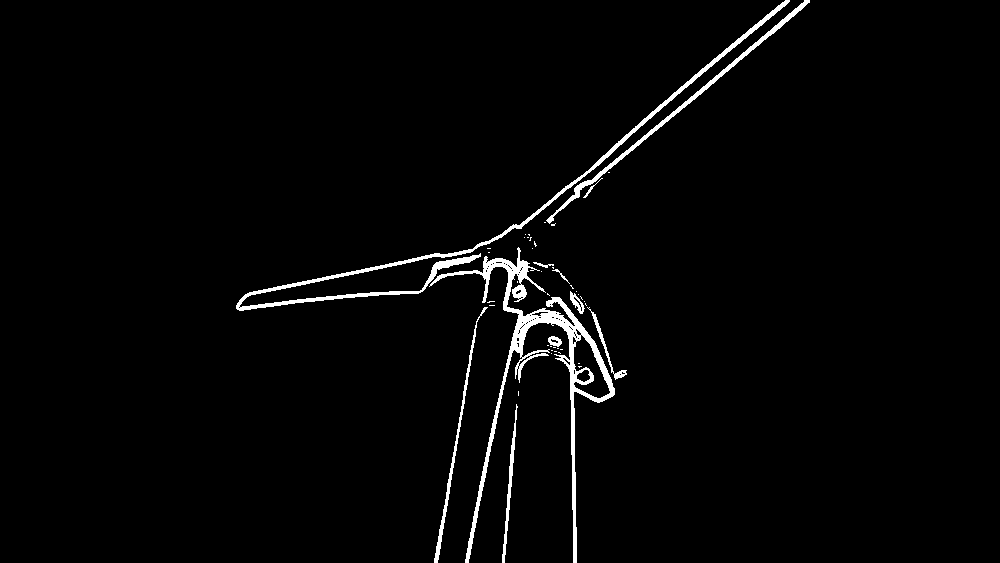
\includegraphics[width=0.42\textwidth]{results/molino_haralick.png}}
	\caption{Results of the Marr-Hildreth and the Haralick algorithms, using the figure \ref{fig:original2} as input image.}
	\label{fig:result3}
\end{figure}

\begin{table}[h!]
	\begin{center}
	\begin{tabular}{| l | r |}
		\hline \rule{0pt}{3ex}
		\cellcolor[gray]{0.8} \textbf{Algorithm}	& \cellcolor[gray]{0.8} \textbf{Execution time (s)}	\\ \hline \rule{0pt}{3ex}
		Roberts, Prewitt and Sobel					& $0.550 \ s$										\\ \hline \rule{0pt}{3ex}
		Marr-Hildreth (Gaussian)					& $1.050 \ s$										\\ \hline \rule{0pt}{3ex}
		Marr-Hildreth (LoG)							& $1.440 \ s$										\\ \hline \rule{0pt}{3ex}
		Haralick									& $0.930 \ s$										\\
		\hline
	\end{tabular}
	\end{center}
	\caption{Execution time of the algorithms using the figure \ref{fig:original2} as input image (1000$\times$563 pixels, 3 channels).}
	\label{exectime2}
\end{table}
\vspace{0.5cm}

It is now visible the difference in performance between the first derivative edge detection algorithms and the second derivative ones. \\

\clearpage
%-------------------------------------------------------------------------------
\section{Conclusions}
\label{sec:conclusions}


\clearpage
%-------------------------------------------------------------------------------
\section{Appendix: Common operations}
\label{sec:appendix1}

All algorithms implemented use some common operations that are independent of the algorithms themselves. 
These operations, although basic, have a great impact on the algorithm outcome, and thus they need to be 
implemented with care.\\

\subsection{Grayscale conversion}

The first step in every algorithm presented above is to convert color images to gray intensity images. 
We use the libpng coefficients to do this:
\begin{equation}
    Y = (6968 R + 23434 G + 2366 B) / 32768
\end{equation}
where $R$, $G$ and $B$ are the red, green and blue components respectively.\\

%-------------------------------------------------------------------------------
\subsection{Kernel generation}
\label{sec:appendix2}

Some of the algorithms presented above require the use of a Gaussian kernel or a LoG kernel. These 
kernels are generated by sampling the corresponding analytical function, which in each case depends 
on the parameter $\sigma$ (standard deviation of the Gaussian function). The result is an array of 
size $n$ by $n$.\\

\subsubsection{Gaussian kernel}

We generate the Gaussian kernel by sampling the 2-D Gaussian function\footnote{Note that for simplicity 
we omitted the normalizing coefficient $1/\sqrt{2\pi\sigma^2}$.}
\begin{equation}
	\label{eq:gaussian_function}
	G(x,y) = e^{-\frac{x^2+y^2}{2\sigma^2}}
\end{equation}
where $\sigma$ is the standard deviation (sometimes $\sigma$ is called the \textit{space constant}).\\

The size of the kernel $n$ and the standard deviation of the exponential function $\sigma$ are both 
input parameters, but these are not strictly independent of each other. We need a value 
of $n$ large enough to ensure that no information is lost when creating the kernel $G$. To ensure this, we take 
$n$ equal to the first odd integer greater than $6\sigma$. Larger values of $n$ does not add more 
significant samples ​​of $G$, and increases the number of operations in the convolution.\\

Figure \ref{fig:gaussian_kernel} shows a Gaussian kernel, generated with $\sigma = 4$ and $n = 25$ 
(first odd integer greater than $6\sigma=24$).\\

\begin{SCfigure}[][!t]
	\centering
	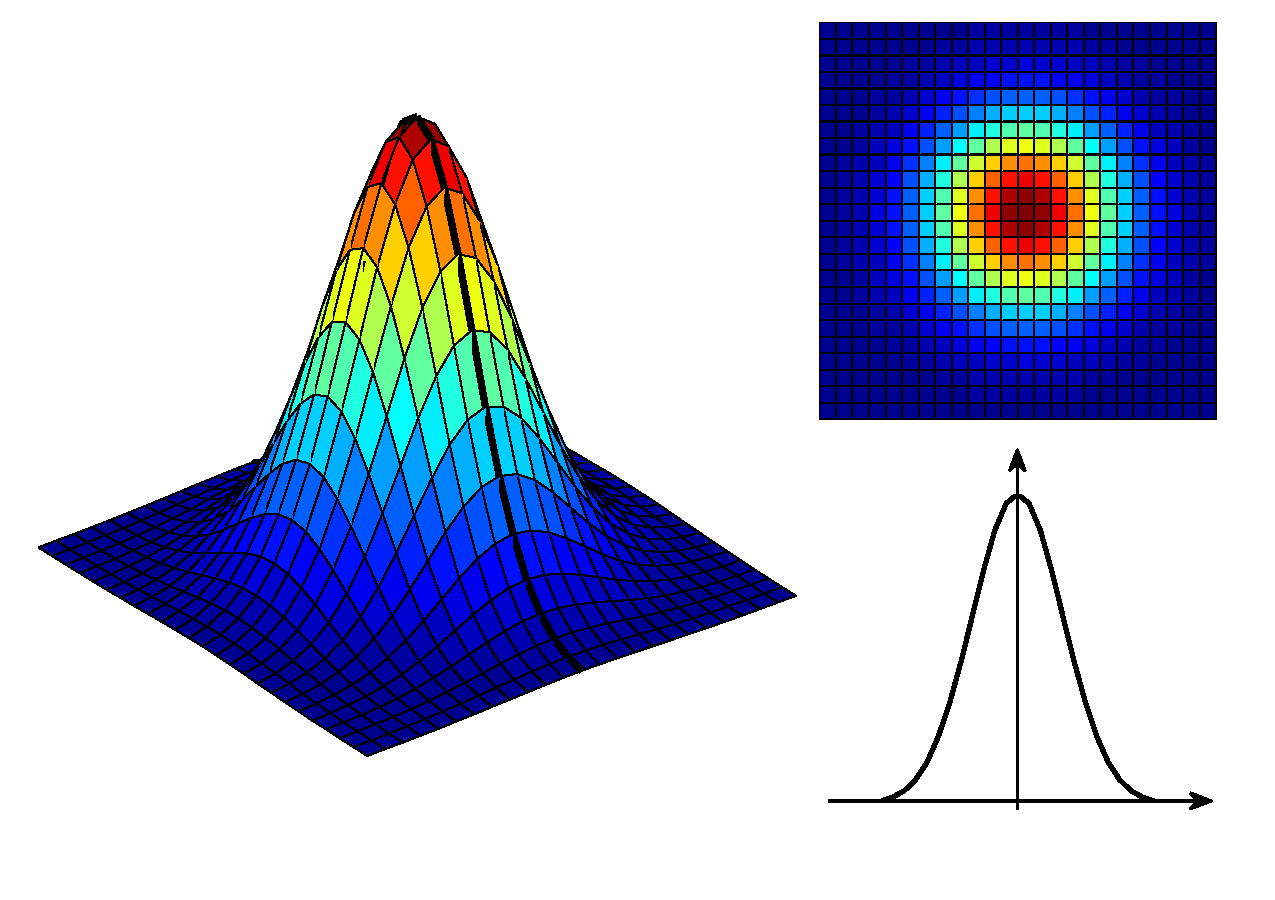
\includegraphics[width=0.5\textwidth]{kernel_gaussian.pdf}
	\caption{Gaussian kernel, $\sigma=4$, $n=25$. Is easy to see that the selected value of n is 
sufficient to have a good approximation of the Gaussian function in the kernel.}
	\label{fig:gaussian_kernel}
\end{SCfigure}

\subsubsection{LoG kernel}

We can obtain analytically the Laplacian of Gaussian $\nabla^2G(x,y)$ first, and generate a kernel 
with the result function. Use this kernel for edge detection involves only one convolution with 
the input image (unlike the case of Gaussian kernel, where we have to make two convolutions, one 
with the kernel and another with the Laplacian operator).\\

\begin{equation}
	LoG \stackrel{\triangle}{=}\nabla^2G(x,y)=\frac{\partial^2}{\partial^2 x}G(x,y) + \frac{\partial^2}{\partial^2 y}G(x,y)
\end{equation}

We first obtain:

\begin{equation} 
	\frac{\partial}{\partial x}G(x,y)=-\frac{x}{\sigma^2}e^{-(x^2+y^2)/2\sigma^2}
\end{equation}

And then:

\begin{equation} 
	\frac{\partial^2}{\partial^2 x}G(x,y)=\frac{x^2-\sigma^2}{\sigma^4}e^{-(x^2+y^2)/2\sigma^2} 
\end{equation}

Similarly:

\begin{equation} 
	\frac{\partial^2}{\partial^2 y}G(x,y)=\frac{y^2-\sigma^2}{\sigma^4}e^{-(x^2+y^2)/2\sigma^2} 
\end{equation}

Therefore we obtain:

\begin{equation}
	\label{eq:log_function}
	LoG(x,y)=\frac{x^2+y^2-2\sigma^2}{\sigma^4}e^{-(x^2+y^2)/2\sigma^2}
\end{equation}\\

Now we generate the LoG kernel by sampling this function. Figure \ref{fig:log_kernel} shows a LoG kernel, generated using the 
values $\sigma=4$ and $n=31$.\\

\begin{SCfigure}[][!t]
	\centering
	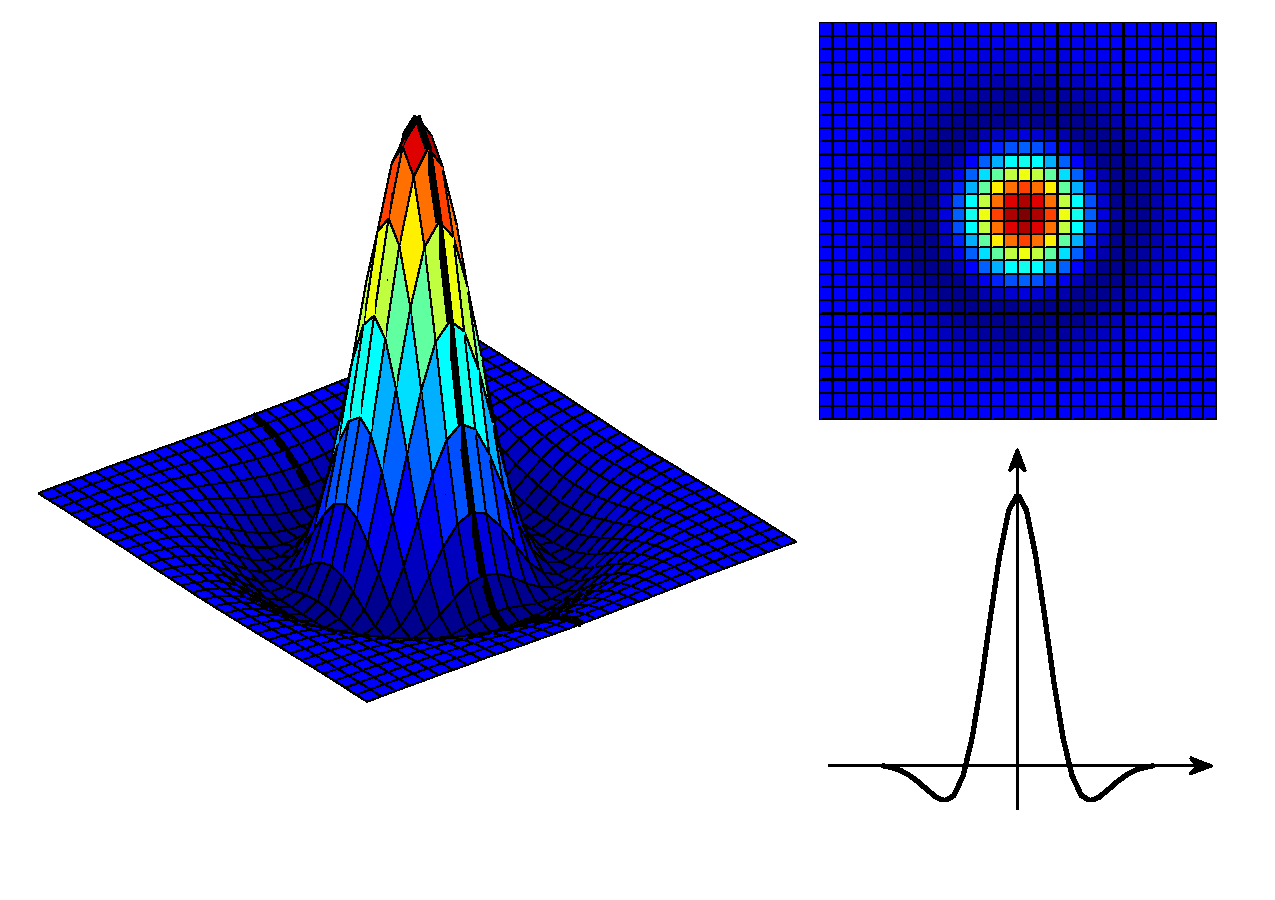
\includegraphics[width=0.5\textwidth]{kernel_log.pdf}
	\caption{Laplacian of a Gaussian kernel, $\sigma=4$, $n=31$. The selected value of n is sufficient 
to have a good approximation of the LoG function in the kernel, but is greater than in the case of 
Gaussian kernel.}
	\label{fig:log_kernel}
\end{SCfigure}

\subsubsection{Gaussian and LoG functions comparison}

As we said before, the size of the kernel $n$ and the standard deviation of the exponential function 
$\sigma$ are not independent of each one. This is because the function LoG is "wider" that the 
Gaussian function (i.e. LoG function has a slower decay), so we need a greater value of $n$ to 
generate a correctly sampled LoG kernel than the needed in the case of the Gaussian kernel, with the same $\sigma$.\\

Figure \ref{fig:kernels} shows both functions generated with the same value of $\sigma$. Is clearly 
required a larger kernel size in the case of the LoG function (approximately 18\% more). For 
example, using $\sigma=4$, the optimum value for $n$ in the case of the Gaussian function is the 
first odd integer greater than $6*\sigma$, which is $25$, and for the case of LoG function, would 
be $29$.\\

\begin{SCfigure}[][!t]
	\centering
	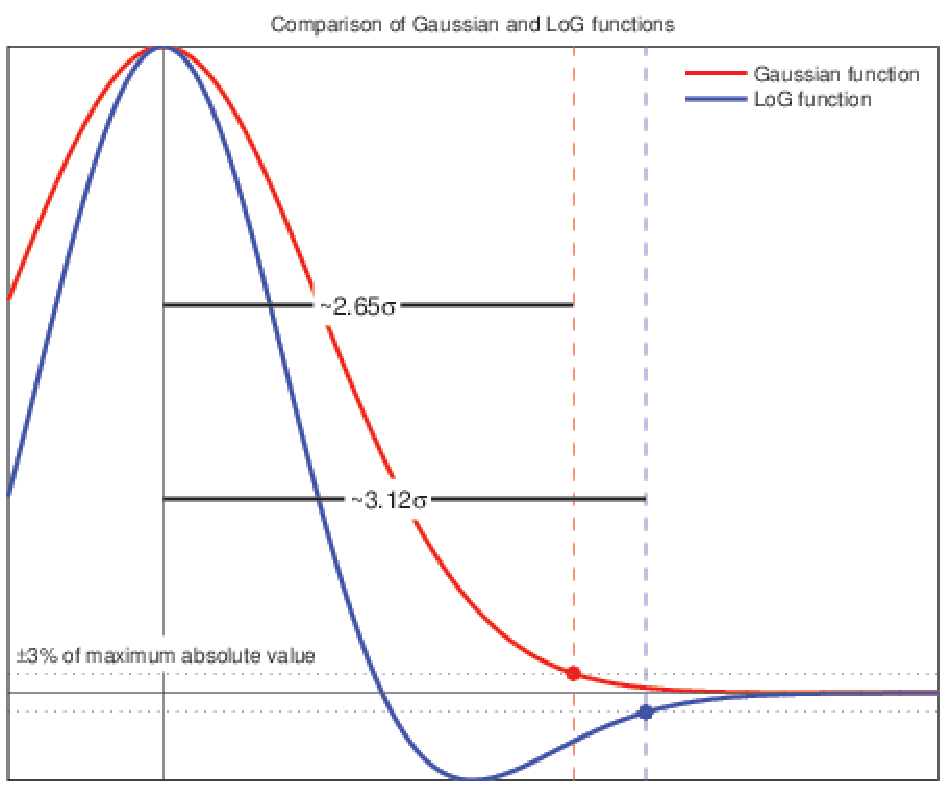
\includegraphics[width=0.5\textwidth]{kernels.pdf}
	\caption{Comparison of the Gaussian and LoG functions.}
	\label{fig:kernels}
\end{SCfigure}

\clearpage
%-------------------------------------------------------------------------------
\section{Examples}
\label{sec:examples}

\subsection{Images}

Further examples obtained with the implemented algorithms are shown in figures \ref{fig:example1} to \ref{fig:example3}. More examples can be found in the online demo. \\

\begin{figure}[h!]
	\centering
	\subfloat[Roberts.]{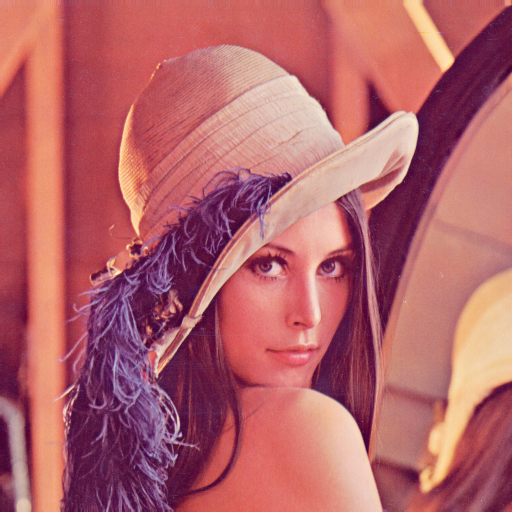
\includegraphics[width=0.3\textwidth]{examples/lena.png}}

	\subfloat[Roberts.]{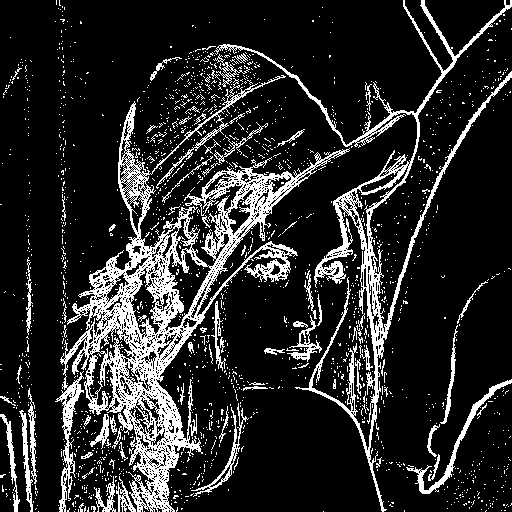
\includegraphics[width=0.3\textwidth]{examples/lena_roberts.png}}
	\quad
	\subfloat[Prewitt.]{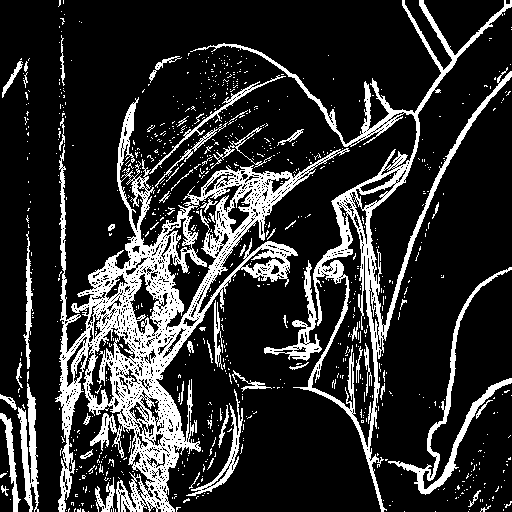
\includegraphics[width=0.3\textwidth]{examples/lena_prewitt.png}}
	\quad
	\subfloat[Sobel.]{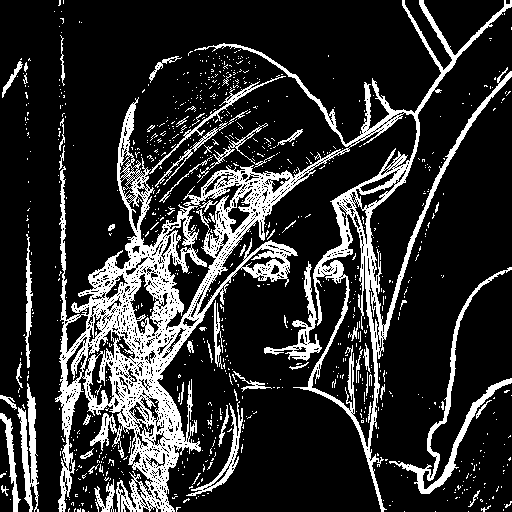
\includegraphics[width=0.3\textwidth]{examples/lena_sobel.png}}

	\subfloat[Marr-Hildreth (Gaussian).]{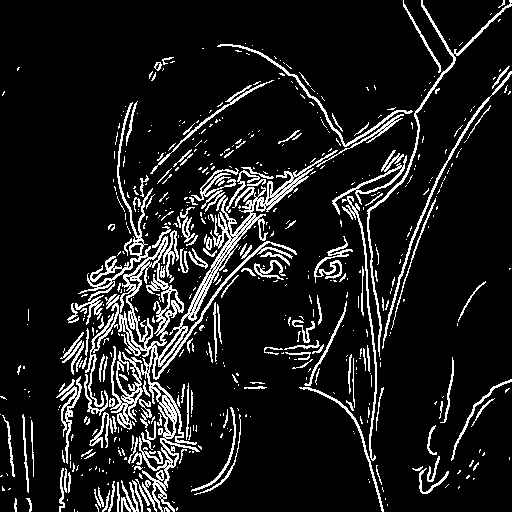
\includegraphics[width=0.3\textwidth]{examples/lena_marr-hildreth.png}}
	\quad
	\subfloat[Marr-Hildreth (LoG).]{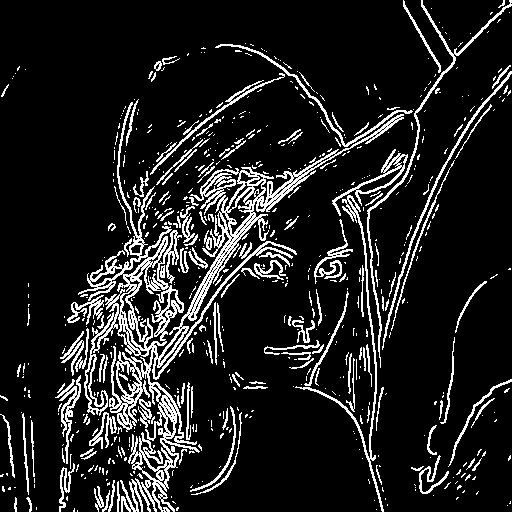
\includegraphics[width=0.3\textwidth]{examples/lena_marr-hildreth-log.png}}
	\quad
	\subfloat[Haralick.]{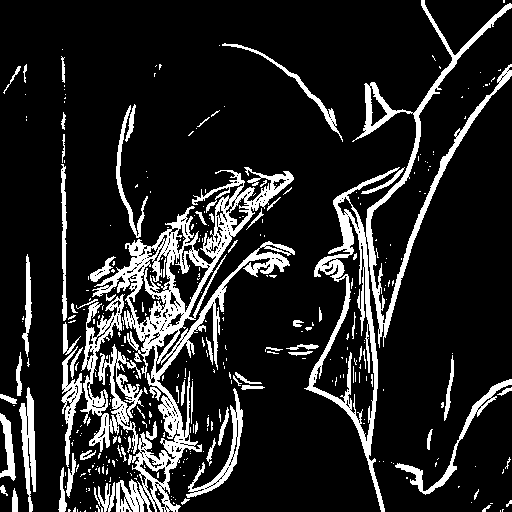
\includegraphics[width=0.3\textwidth]{examples/lena_haralick.png}}
	\caption{Example: Lena.}
	\label{fig:example1}
\end{figure}

\begin{figure}[t!]
	\centering
	\subfloat[Roberts.]{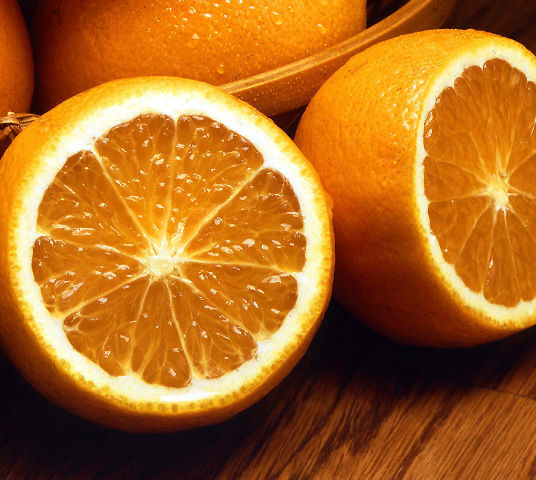
\includegraphics[width=0.3\textwidth]{examples/oranges.png}}

	\subfloat[Roberts.]{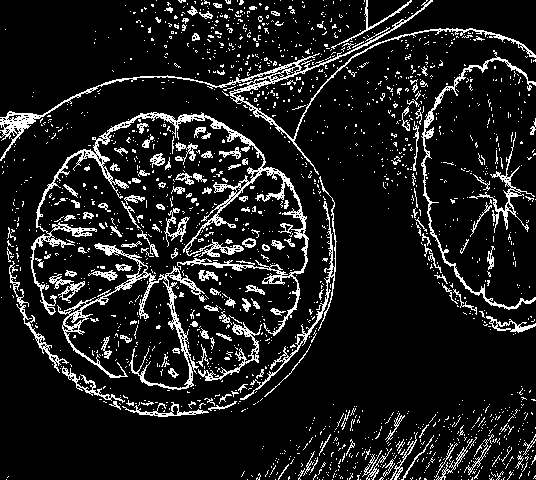
\includegraphics[width=0.3\textwidth]{examples/oranges_roberts.png}}
	\quad
	\subfloat[Prewitt.]{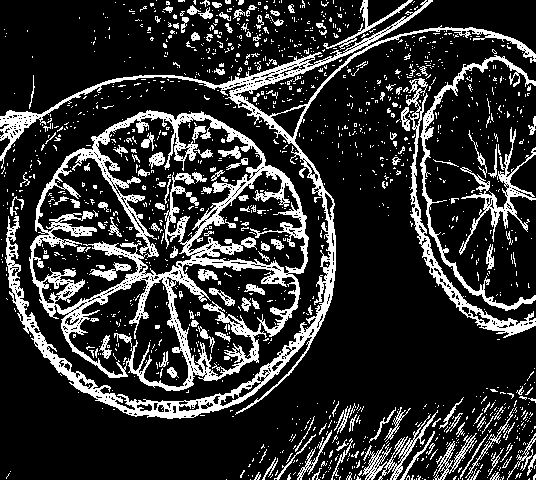
\includegraphics[width=0.3\textwidth]{examples/oranges_prewitt.png}}
	\quad
	\subfloat[Sobel.]{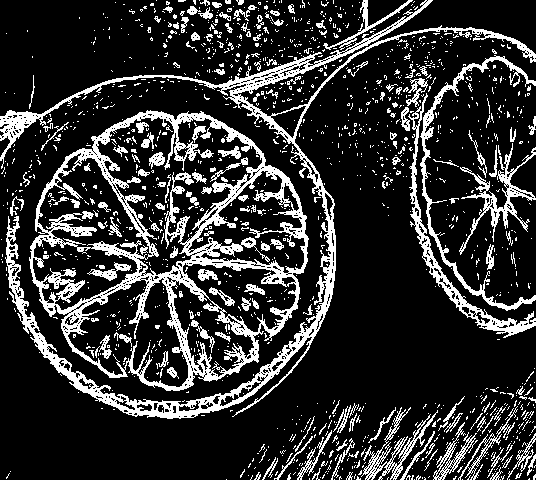
\includegraphics[width=0.3\textwidth]{examples/oranges_sobel.png}}

	\subfloat[Marr-Hildreth (Gaussian).]{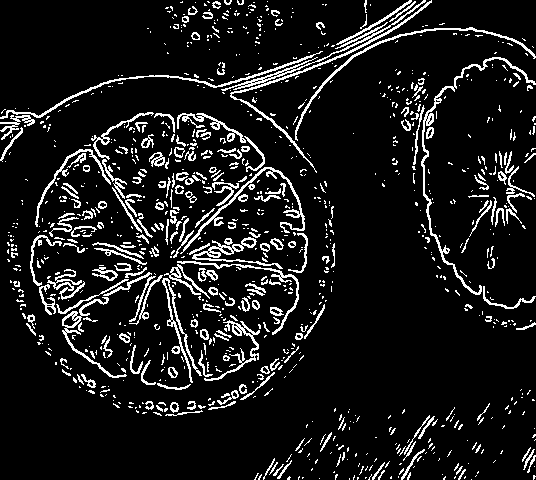
\includegraphics[width=0.3\textwidth]{examples/oranges_marr-hildreth.png}}
	\quad
	\subfloat[Marr-Hildreth (LoG).]{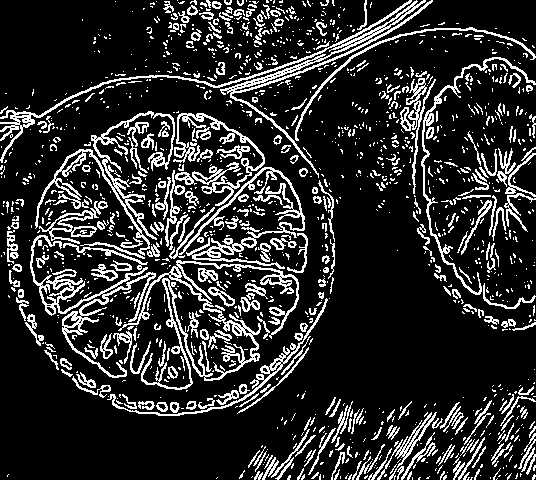
\includegraphics[width=0.3\textwidth]{examples/oranges_marr-hildreth-log.png}}
	\quad
	\subfloat[Haralick.]{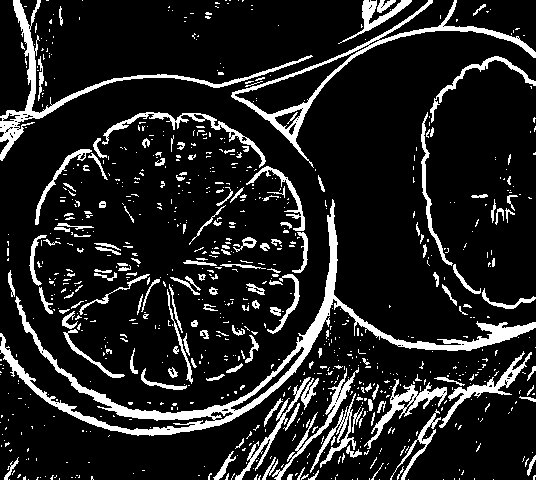
\includegraphics[width=0.3\textwidth]{examples/oranges_haralick.png}}
	\caption{Example: Oranges.}
	\label{fig:example2}
\end{figure}

\vspace{2cm}

\begin{figure}[t!]
	\centering
	\subfloat[Roberts.]{\includegraphics[width=0.3\textwidth]{examples/shapes.png}}

	\subfloat[Roberts.]{\includegraphics[width=0.3\textwidth]{examples/shapes_roberts.png}}
	\quad
	\subfloat[Prewitt.]{\includegraphics[width=0.3\textwidth]{examples/shapes_prewitt.png}}
	\quad
	\subfloat[Sobel.]{\includegraphics[width=0.3\textwidth]{examples/shapes_sobel.png}}

	\subfloat[Marr-Hildreth (Gaussian).]{\includegraphics[width=0.3\textwidth]{examples/shapes_marr-hildreth.png}}
	\quad
	\subfloat[Marr-Hildreth (LoG).]{\includegraphics[width=0.3\textwidth]{examples/shapes_marr-hildreth-log.png}}
	\quad
	\subfloat[Haralick.]{\includegraphics[width=0.3\textwidth]{examples/shapes_haralick.png}}
	\caption{Example: Shapes.}
	\label{fig:example3}
\end{figure}

%-------------------------------------------------------------------------------
\subsection{Video}

%TODO: videos de ejemplo con todos los métodos.

This is an example of applying the edge detection algorithms described here, frame by frame, to a video: 
\begin{itemize}
	\centering
	\item \href{http://iie.fing.edu.uy/~haldos/ipol/video.mov}{original} (xxxMb).
\end{itemize}
\begin{multicols}{2}
\begin{itemize}
	\item \href{http://iie.fing.edu.uy/~haldos/ipol/video-roberts.mov}{roberts version} (xxxMb).
	\item \href{http://iie.fing.edu.uy/~haldos/ipol/video-prewitt.mov}{prewitt version} (xxxMb).
	\item \href{http://iie.fing.edu.uy/~haldos/ipol/video-sobel.mov}{sobel version} (xxxMb).
	\item \href{http://iie.fing.edu.uy/~haldos/ipol/video-marr-hildreth-gaussian.mov}{marr-hildreth-gaussian version} (xxxMb).
	\item \href{http://iie.fing.edu.uy/~haldos/ipol/video-marr-hildreth-log.mov}{marr-hildreth-log version} (xxxMb).
	\item \href{http://iie.fing.edu.uy/~haldos/ipol/video-haralick.mov}{haralick version} (xxxMb).
\end{itemize}
\end{multicols}

%-------------------------------------------------------------------------------
\begin{thebibliography}{9}

\end{thebibliography}

\end{document}
%-------------------------------------------------------------------------------
